%!TEX root = ../../../_main.tex
\subsection{Twisted weak ordering}
\label{sec:twisted-involutions-twisted-weak-ordering}

In this section we introduce the twisted weak ordering $Wk(\theta)$ on the set $\ti{\theta}$ of $\theta$-twisted involutions.

\begin{defi}
	We define the set of \defword{$\theta$-twisted involutions} as $\{ w \in W : \theta(w) = w^{-1} \}$, denoted by $\ti{\theta}$. If $\theta$ is clear from the context we just say \defword{twisted involutions}. Every element $w \in \ti{\theta}$ is called a $\theta$-twisted involution, resp. twisted involution.
\end{defi}

\begin{defi}
	For $v,w \in \ti{\theta}$ we define $v \preceq w$ iff there are $\ul s_1, \ldots, \ul s_k \in \ul S$ with $w = v \ul s_1 \ldots \ul s_k$ and $\rho(v) = \rho(w) - k$. We call the poset $(\ti{\theta},\preceq)$ \defword{twisted weak ordering}, denoted by $Wk(W, \theta)$. When the Coxeter group $W$ is clear from the context, we just write $Wk(\theta)$.
\end{defi}

\begin{lemm}
	The poset $Wk(\theta)$ is a graded poset with rank function $\rho$.

	\begin{proof}
		Follows immediately from the definition of $\preceq$.
	\end{proof}
\end{lemm}

By a diagram of a poset $Wk(\theta)$, we do not just mean the ordinary Hasse diagram. Suppose $w,v \in Wk(\theta)$ with $w \ul s = v$. We encode the information, if $s$ acts as twisted involution or as multiplication on $w$, by drawing either a solid or a dashed edge from $w$ to $v$. For simplification of terminology we still just speak of the Hasse diagram of $Wk(\theta)$. The next example shows such a (extended) Hasse diagram.

\begin{exam}
	In Figure \ref{fig:a4} we see the Hasse diagram of $Wk(A_4, \id)$. Solid edges represent twisted congujations and dashed edges represent multiplications.
	\begin{figure}[ht]
		\centering
		%!TEX root = ../../_main.tex
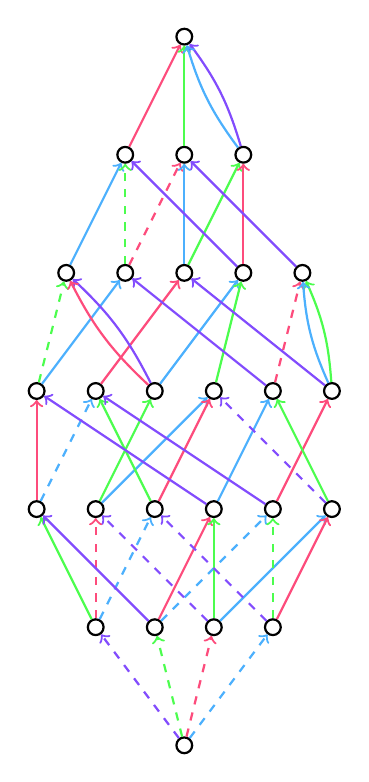
\begin{tikzpicture}[scale=1,bend angle=10]
\newcommand{\xspace}{1}
\newcommand{\yspace}{1}
\tikzstyle{vertex}=[draw,thick,circle,minimum size=2mm,inner sep=0pt]
\tikzstyle{edge}=[thick,->]
\tikzstyle{onesided}=[edge,dashed]
\tikzstyle{bothsided}=[edge]
\tikzstyle{unhighlighted}=[]
\tikzstyle{highlighted}=[]
\definecolor{s1color}{RGB}{130,76,253}
\definecolor{s2color}{RGB}{76,253,78}
\definecolor{s3color}{RGB}{253,76,124}
\definecolor{s4color}{RGB}{76,176,253}
\tikzstyle{s1}=[s1color]
\tikzstyle{s2}=[s2color]
\tikzstyle{s3}=[s3color]
\tikzstyle{s4}=[s4color]
\node[vertex,unhighlighted] (0) at (\xspace*0,\yspace*0) {};
\node[vertex,unhighlighted] (1) at (\xspace*-1.125,\yspace*1.5) {};
\node[vertex,unhighlighted] (2) at (\xspace*-0.375,\yspace*1.5) {};
\node[vertex,unhighlighted] (3) at (\xspace*0.375,\yspace*1.5) {};
\node[vertex,unhighlighted] (4) at (\xspace*1.125,\yspace*1.5) {};
\node[vertex,unhighlighted] (5) at (\xspace*-1.875,\yspace*3) {};
\node[vertex,unhighlighted] (6) at (\xspace*-1.125,\yspace*3) {};
\node[vertex,unhighlighted] (7) at (\xspace*-0.375,\yspace*3) {};
\node[vertex,unhighlighted] (8) at (\xspace*0.375,\yspace*3) {};
\node[vertex,unhighlighted] (9) at (\xspace*1.125,\yspace*3) {};
\node[vertex,unhighlighted] (10) at (\xspace*1.875,\yspace*3) {};
\node[vertex,unhighlighted] (11) at (\xspace*-1.875,\yspace*4.5) {};
\node[vertex,unhighlighted] (12) at (\xspace*-1.125,\yspace*4.5) {};
\node[vertex,unhighlighted] (13) at (\xspace*-0.375,\yspace*4.5) {};
\node[vertex,unhighlighted] (14) at (\xspace*0.375,\yspace*4.5) {};
\node[vertex,unhighlighted] (15) at (\xspace*1.125,\yspace*4.5) {};
\node[vertex,unhighlighted] (16) at (\xspace*1.875,\yspace*4.5) {};
\node[vertex,unhighlighted] (17) at (\xspace*-1.5,\yspace*6) {};
\node[vertex,unhighlighted] (18) at (\xspace*-0.75,\yspace*6) {};
\node[vertex,unhighlighted] (19) at (\xspace*0,\yspace*6) {};
\node[vertex,unhighlighted] (20) at (\xspace*0.75,\yspace*6) {};
\node[vertex,unhighlighted] (21) at (\xspace*1.5,\yspace*6) {};
\node[vertex,unhighlighted] (22) at (\xspace*-0.75,\yspace*7.5) {};
\node[vertex,unhighlighted] (23) at (\xspace*0,\yspace*7.5) {};
\node[vertex,unhighlighted] (24) at (\xspace*0.75,\yspace*7.5) {};
\node[vertex,unhighlighted] (25) at (\xspace*0,\yspace*9) {};
\draw[s1,onesided,unhighlighted] (0) edge (1);
\draw[s2,onesided,unhighlighted] (0) edge (2);
\draw[s3,onesided,unhighlighted] (0) edge (3);
\draw[s4,onesided,unhighlighted] (0) edge (4);
\draw[s2,bothsided,unhighlighted] (1) edge (5);
\draw[s3,onesided,unhighlighted] (1) edge (6);
\draw[s4,onesided,unhighlighted] (1) edge (7);
\draw[s1,bothsided,unhighlighted] (2) edge (5);
\draw[s3,bothsided,unhighlighted] (2) edge (8);
\draw[s4,onesided,unhighlighted] (2) edge (9);
\draw[s1,onesided,unhighlighted] (3) edge (6);
\draw[s2,bothsided,unhighlighted] (3) edge (8);
\draw[s4,bothsided,unhighlighted] (3) edge (10);
\draw[s1,onesided,unhighlighted] (4) edge (7);
\draw[s2,onesided,unhighlighted] (4) edge (9);
\draw[s3,bothsided,unhighlighted] (4) edge (10);
\draw[s3,bothsided,unhighlighted] (5) edge (11);
\draw[s4,onesided,unhighlighted] (5) edge (12);
\draw[s2,bothsided,unhighlighted] (6) edge (13);
\draw[s4,bothsided,unhighlighted] (6) edge (14);
\draw[s2,bothsided,unhighlighted] (7) edge (12);
\draw[s3,bothsided,unhighlighted] (7) edge (14);
\draw[s1,bothsided,unhighlighted] (8) edge (11);
\draw[s4,bothsided,unhighlighted] (8) edge (15);
\draw[s1,bothsided,unhighlighted] (9) edge (12);
\draw[s3,bothsided,unhighlighted] (9) edge (16);
\draw[s1,onesided,unhighlighted] (10) edge (14);
\draw[s2,bothsided,unhighlighted] (10) edge (15);
\draw[s2,onesided,unhighlighted] (11) edge (17);
\draw[s4,bothsided,unhighlighted] (11) edge (18);
\draw[s3,bothsided,unhighlighted] (12) edge (19);
\draw[s1,bothsided,unhighlighted,bend right] (13) edge (17);
\draw[s3,bothsided,unhighlighted,bend left] (13) edge (17);
\draw[s4,bothsided,unhighlighted] (13) edge (20);
\draw[s2,bothsided,unhighlighted] (14) edge (20);
\draw[s1,bothsided,unhighlighted] (15) edge (18);
\draw[s3,onesided,unhighlighted] (15) edge (21);
\draw[s1,bothsided,unhighlighted] (16) edge (19);
\draw[s2,bothsided,unhighlighted,bend right] (16) edge (21);
\draw[s4,bothsided,unhighlighted,bend left] (16) edge (21);
\draw[s4,bothsided,unhighlighted] (17) edge (22);
\draw[s2,onesided,unhighlighted] (18) edge (22);
\draw[s3,onesided,unhighlighted] (18) edge (23);
\draw[s4,bothsided,unhighlighted] (19) edge (23);
\draw[s2,bothsided,unhighlighted] (19) edge (24);
\draw[s1,bothsided,unhighlighted] (20) edge (22);
\draw[s3,bothsided,unhighlighted] (20) edge (24);
\draw[s1,bothsided,unhighlighted] (21) edge (23);
\draw[s3,bothsided,unhighlighted] (22) edge (25);
\draw[s2,bothsided,unhighlighted] (23) edge (25);
\draw[s1,bothsided,unhighlighted,bend right] (24) edge (25);
\draw[s4,bothsided,unhighlighted,bend left] (24) edge (25);
\end{tikzpicture}
		\caption{Hasse diagram of $Wk(A_4, \id)$}
		\label{fig:a4}
	\end{figure}
\end{exam}

\begin{lemm}
	\typedlabel{lemm:wk-subposet-of-br}
	The poset $Wk(\theta)$ is a subposet of $\Br(\ti{\theta})$.

	\begin{proof}
		Both posets are defined on $\ti{\theta}$. Let $w,v \in \ti{\theta}$ be two twisted involutions. Assume $w \preceq v$ with $w \ul s = v$ for some $s \in S$. If $\ul s$ acts by multiplication on $w$, then $ws = v$ and since $s \in T$ ($T$ the set of all reflections in $W$) and $l(w \ul s) = l(w) + 1$ we have $w \leq v$. If conversely $\ul s$ acts by twisted conjugation on $w$, then $v = \theta(s)ws = w (w^{-1} \theta(s) w)(e^{-1}se)$ and since $w^{-1} \theta(s) w, s \in T$ and $l(w \ul s) = l(\theta(s)w) + 1 = l(w) + 2$ we have again $w \leq v$.
	\end{proof}
\end{lemm}

\begin{prop}
	\typedlabel{prop:w-ul-s-leq-w-iff-s-in-dr-w}
	For all $w \in \ti{\theta}$ and $s \in S$ we have $w \ul s \prec w$ iff $s \in D_R(w)$ and $w \ul s \succ w$ iff $s \notin D_R(w)$ as well as $w \ul s < w$ iff $s \in D_R(w)$ and $w \ul s > w$ iff $s \notin D_R(w)$.

	\begin{proof}
		We have $w \ul s \ul s = w$ and $\rho(w \ul s) = \rho(w) - 1$ iff $s \in D_R(w)$ and $\rho(w \ul s) = \rho(w) + 1$ iff $s \notin D_R(w)$ by \ref{lemm:rho-w-ul-s-minus-rho-w-differs-by-1}. By \ref{lemm:wk-subposet-of-br} both statements are true for $\Br(\ti{\theta})$, too.
	\end{proof}
\end{prop}

\begin{defi}
	Let $v,w \in W$ with $\rho(w) - \rho(v) = n$. A sequence $v = w_0 \prec w_1 \prec \ldots \prec w_n = w$ is called a \defword{geodesic} from $v$ to $w$.
\end{defi}

\begin{prop}
	\typedlabel{prop:geodesics-have-same-count-of-multiplicative-steps}
	Let $v,w \in W$ with $v \prec w$. Then all geodesics from $v$ to $w$ have the same count of twisted conjugated and multiplicative steps.

	\begin{proof}
		Suppose we have two geodesics from $v$ to $w$, where the first has $n$ and the second $m$ multiplicative steps. Then $l(w) + n + 2(k-n) = l(v) = l(w) + m + 2(k-m)$, hence $n = m$.
	\end{proof}
\end{prop}

\begin{prop}
	\typedlabel{prop:no-triple-edges}
	Let $w \in W$ and $w \ul s \succ w$. Then $|\{ t \in S \setminus D_R(w) : w \ul t = w \ul s \}| \in \{1,2\}$.

	\begin{proof}
		Suppose $t \in S \setminus D_R(w)$ with $w \ul t = w \ul s$. Because of the ordinary length either both $\ul s$ and $\ul t$ act by multiplication on $w$, or both act by twisted conjugation on $w$. Suppose they act by multiplication, then $ws = w \ul s = w \ul t = wt$, hence $s = t$. Conversely, assume they act by twisted conjugation. Then $\theta(s) w s = w \ul s = w \ul t = \theta(t)wt$. Because of $\theta(t) w t t = \theta(t) w = \theta(s) w s t$ we have $l(\theta(s) w s t) < l(\theta(s) w s)$ and so by \ref{coro:exchange-condition} there are three possible cases
		$$ \theta(t)w = \theta(s) w s t = \begin{cases}
			\theta(s) w & \Rightarrow s = t, \\
			w s & \Rightarrow \theta(t) = w s w^{-1} \textrm{ or} \\
			\theta(s) \overline w s & \Rightarrow w = \theta(t) \theta(s) \overline w s, \\
		\end{cases} $$
		where $\overline w$ denotes a well choosen subexpression of $w$. The first case is trivial, the second determines $t$ unambiguously. The third case is impossible, since by \ref{coro:exchange-condition} and \ref{rema:exchange-condition-left-sided} we would have a reduced expression for $w$ beginning with $\theta(s)$ or ending with $s$ (or both), yielding $l(\theta(s)ws) \leq l(w)$, which contradicts to $\rho(w \ul s) = \rho(\theta(s)ws) > \rho(w)$. Therefore, there cannot be more than two distinct $s,t \in S \setminus D_R(w)$ with $w \ul s = w \ul t$.
	\end{proof}
\end{prop}

\begin{coro}
	\typedlabel{coro:double-edges-only-for-ord-2}
	Let $w \in \ti{\theta}$ and $s,t \in S$ be two distinct generators. If $w \ul s = w \ul t$, then $\ord(st) = 2$.

	\begin{proof}
		By the proof of \ref{prop:no-triple-edges} we see, that $w \ul s = w \ul t$ for two distinct $s,t \in S$ implies, that $\theta(t)w = ws$ holds and that $\ul s$ and $\ul t$ act by twisted conjugation on $w$. Since $\theta(w) = w^{-1}$, we also have $\theta(s)w = wt$ by
		$$ \theta(t)w = ws \iff \theta(\theta(t)w) = \theta(ws) \iff tw^{-1} = w^{-1} \theta(s) \iff wt = \theta(s)w. $$
		Hence we have $wts = \theta(s)ws = \theta(t)wt = wst$, yielding $st = ts$ and $\ord(st) = 2$.
	\end{proof}
\end{coro}

\todo